\documentclass[
    %aspectratio=169,
]{beamer}

\usepackage[english]{babel}
\usepackage[utf8]{inputenc}
\usepackage[T1]{fontenc}
\usepackage{csquotes}
\usepackage{expl3,biblatex}

\addbibresource{bibliography.bib}

\usepackage{booktabs}
\usetheme{Madrid}
\usecolortheme{crane}
\usepackage{svg}
\usepackage{graphicx,caption}

% set font
\usefonttheme{serif}

% to prevent the boxes from overlapping the logo at the lower right corner
\addtobeamertemplate{block begin}{%
  \setlength{\textwidth}{0.9\textwidth}%
}{}

\addtobeamertemplate{block alerted begin}{%
  \setlength{\textwidth}{0.9\textwidth}%
}{}

\addtobeamertemplate{block example begin}{%
  \setlength{\textwidth}{0.9\textwidth}%
}{}


% usage: \hl{text to emphasis as yellow background}
\usepackage{soul}
\makeatletter
\let\HL\hl
\renewcommand\hl{%
  \let\set@color\beamerorig@set@color
  \let\reset@color\beamerorig@reset@color
  \HL}
\makeatother


% usage: create outline pages before each section
\AtBeginSection[]
{
  \begin{frame}
    \frametitle{Table of Contents}
    \tableofcontents[currentsection]
  \end{frame}
}

% Title page information
\title[Mid-Project Update]{Preschooler Data}
\subtitle[Short Subtitle]{STATS 570/409}
\author[Data Whisperers]{Lauren, Will, Betsy, Ryan\texorpdfstring{\\}{, }wmm2@pdx.edu}
\institute[PSU]{Portland State University}
\date{April 27, 2023}
\logo{\includesvg[height=1cm]{./uibeamer/logo/ui-stacked-gold-black.svg}}
\subject{Presentation Subject}
\keywords{the, presentation, keywords}

\begin{document}

% make the title page
\begin{frame}%[plain]
\maketitle
\end{frame}

% make the outline page/table of contents
\begin{frame}
\frametitle{Table of Contents}
\tableofcontents
\end{frame}
\section[Short Section 1 Name]{This is the problem.}
\subsection[Short Subsection 1 Name]{Intro to data set}

\begin{frame}{The Dataset}{Preschooler Dataset}
Here is the data set!!!
\begin{figure}[h]
\centering
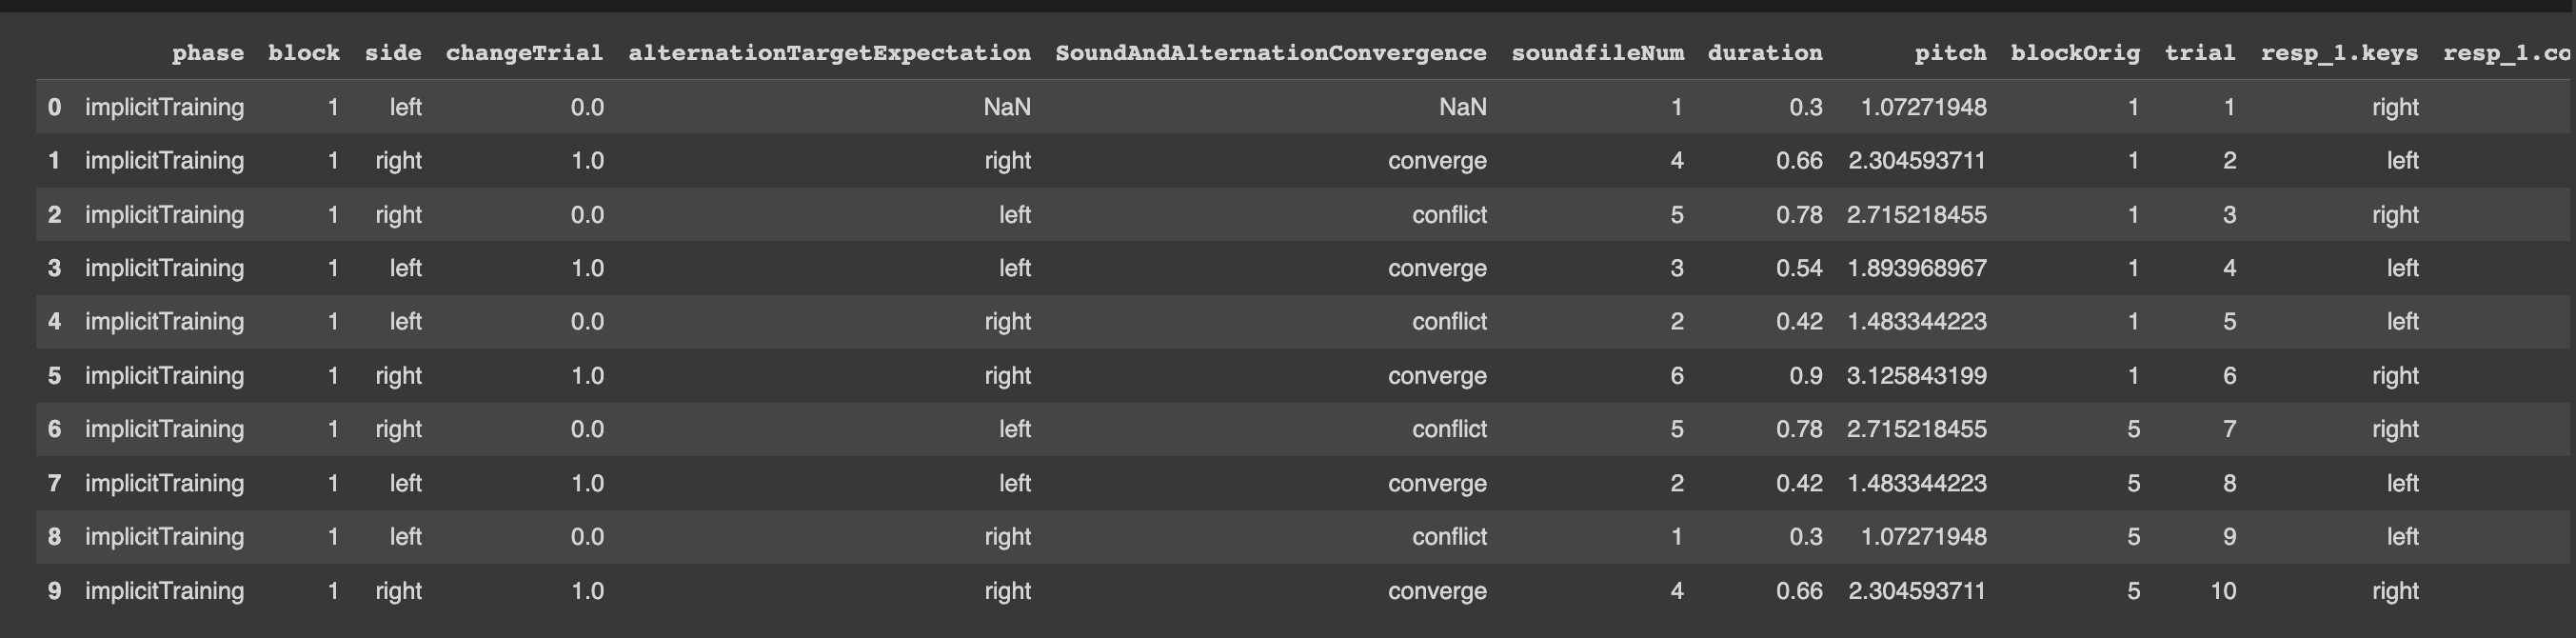
\includegraphics[scale=0.25]{slides/images/dataset.png}
\caption{An example of the data set of awesomeness!!!}
\label{fig:x cubed graph}
\end{figure}

\begin{table}
  \begin{tabular}{llc}
    Category & Item & Quantity \\ \midrule
    A & Item A1 & 15 \\
    A & Item A2 & 20 \\
  \end{tabular}
  \caption{Example data for demonstration purposes}
\end{table}

\end{frame}


\subsection[Short Subsection 2 Name]{Dataset Columns}

\begin{frame}{Columns}
'phase',
 'block',
 'side',
 'changeTrial',
 'alternationTargetExpectation',
 'SoundAndAlternationConvergence',
 'soundfileNum',
 'duration',
 'pitch',
 'blockOrig',
 'trial',
 'resp_1.keys',
 'resp_1.corr',
 'responseAlternation.corr',
 'resp_1.rt',
 'mean',
 'SD',
 'RTwoOutlier',
 'LowOutlier',
 'HighOutlier',
 'anticipationThreshold',
 'additiveAgeRTCorrection',
 'ageCorrection5yrs',
 'anticipated',
 'anticipated5',
 'key_resp_20.keys',
 'key_resp_20.corr',
 'categoryDecision',
 'key_resp_20.rt',
 'participant',
 'group',
 'sex',
 'demographicInfo',
 'soundDimension',
 'trialOrder'
\end{frame}


\begin{frame}{Figures}{"Potatoes."}

\begin{figure}
    \includegraphics[width=.5\textwidth,height=.5\textheight,keepaspectratio]{./figures/a-sketch-of-a-dish-of-potato-from-Idaho-state.jpg}
      \caption{a sketch of a dish of potato from Idaho state%
        \footnote{%
          Do you like famous potatoes?
          They do.
          \cite{evelyn1984potatoes}
        }%
      }

\end{figure}
\end{frame}


\subsection[Short Subsection 3 Name]{Predictor Distributions}


\begin{frame}{Sample Data}

\end{frame}


\section[Equation]{Equation and Explanations}

\begin{frame}{Equation and Explanations}{sample equation}
\textbf{Functionality Representation Model (FRM)} is an abstract method that aims to analyze the significance of various components in a complex system.

$$f(z) = \alpha + \sum^{N}_{i=1}\beta_iz_i$$

In this equation, $z$ symbolizes a data point, $z_i$ denotes the $i^{th}$ component of $z$, and $\beta_i$ represents the influence of component $z_i$ on the system's behavior.
    
\end{frame}

\section{\bibname}
\begin{frame}[t, allowframebreaks]{\bibname}
\printbibliography[heading=none]
\end{frame}


%\miniframesoff


\begin{frame}%[plain]
\vfill
\centerline{Thank You for Your Attention!}
\vfill\vfill
\end{frame}
%\input{sample}

\end{document}


